\documentclass{article}


\usepackage{fancyhdr}
\usepackage{extramarks}
\usepackage{amsmath}
\usepackage{amsthm}
\usepackage{amsfonts}
\usepackage{tikz}
\usepackage[plain]{algorithm}
\usepackage{algpseudocode}
\usepackage{enumerate}
\usepackage{tikz}
\usepackage{listings}
\usepackage{hyperref}
\usepackage{subfigure}
\usepackage[graphicx]{realboxes}
\usepackage{xcolor}
\usepackage{color}



% 代码块高级设置
\lstset{
% basicstyle=\footnotesize,                 % 设置整体的字体大小
showstringspaces=false,                     % 不显示字符串中的空格
frame=single,                               % 设置代码块边框
numbers=left,                               % 在左侧显示行号
% numberstyle=\footnotesize\color{gray},    % 设置行号格式
numberstyle=\color{darkgray},               % 设置行号格式
backgroundcolor=\color{white},              % 设置背景颜色
keywordstyle=\color{blue},                  % 设置关键字颜色
commentstyle=\it\color[RGB]{0,100,0},       % 设置代码注释的格式
stringstyle=\sl\color{red},                 % 设置字符串格式
}

\hypersetup{hidelinks,
	colorlinks=true,
	allcolors=black,
	pdfstartview=Fit,
	breaklinks=true}

%
% Basic Document Settings
%  

\topmargin=-0.45in
\evensidemargin=0in
\oddsidemargin=0in
\textwidth=6.5in
\textheight=9.0in
\headsep=0.25in

\linespread{1.1}

\pagestyle{fancy}
\lhead{}
\chead{\hmwkClass : \hmwkTitle}
\rhead{\firstxmark}
\lfoot{\lastxmark}
\cfoot{\thepage}

\renewcommand\headrulewidth{0.4pt}
\renewcommand\footrulewidth{0.4pt}

\setlength\parindent{0pt}



%
% Homework Details
%   - Title
%   - Due date
%   - Class
%   - Instructor
%   - Class number
%   - Name
%   - Student ID

\newcommand{\hmwkTitle}{Lab 1 Report}
\newcommand{\hmwkDueDate}{Octobor 18th}
\newcommand{\hmwkClass}{Advanced Computer Architecture}
\newcommand{\hmwkClassInstructor}{Professor Chundong Wang}

% 正式选课名单确定之后,根据通知填写所在班级编号

\newcommand{\hmwkAuthorName}{Zhenghong Yu}
\newcommand{\hmwkAuthorMail}{yuzhh1@shanghaitech.edu.cn}
\newcommand{\hmwkAuthorID}{2020533156}


%
% Title Page
%

\title{
    \vspace{2in}
    \textmd{\textbf{\hmwkClass:\\  \hmwkTitle}}\\
    \normalsize\vspace{0.1in}\small{Due\ on\ \hmwkDueDate\ at 11:59am}\\
   \vspace{2in}
}

\author{
	Name: \textbf{\hmwkAuthorName} \\
    Mailbox: \textbf{\hmwkAuthorMail} \\
	Student ID: \hmwkAuthorID}
\date{}

\renewcommand{\part}[1]{\textbf{\large Part \Alph{partCounter}}\stepcounter{partCounter}\\}

\begin{document}

\maketitle
\pagebreak
\tableofcontents

\pagebreak


\subsection{Preknowledge}
The task1 is implemented in the branch \textbf{Task1}, the task2 is implemented in the branch \textbf{Task2}.
\section{Task1}
\subsection{Requirement of Exclusive Cache}
Data only has one copy in the cache, different level of cache do not have intersection data.
\subsection{Analysis of Inclusive Cache Implementation}
The simulatior has already provided a inclusive cache implementation. The author use nested recursion to realize it. \textbf{Cache::getByte()} is used to load the data of the current level cache, if success, read and return the value directly, if not, enter \textbf{Cache::loadBlockFromLowerLevel()} to get the target block from a lower cache, find a victim block and replaced it. \textbf{Cache::setByte()} first confirm whether the writing data is in the current level cache, if yes, modified it and return. If not, first use \textbf{Cache::loadBlockFromLowerLevel()} to load the data to the L1 cache, then modified it.\\
It is a complex implementation since the author tried to realize many functions in a same function interface, which means a smaller change might cause the whole program crash, and actually it is a very dirty work to follow his structure to implement a exclusive cache. So I'll state some new functions while reuse as much his codes as possible.
\subsection{Implementation of Exclusive Cache}
The most important question of a exclusive cache is how to keep the data only one copy in all level of cache. And in my opinion,\\\textbf{First, each time we read a data from memory, we only read it to the L1 cache}. \\\textbf{Second, each time we read a data from L2/L3 cache to L1 cache, we will invalid the old data of the L2/L3 cache}.\\ Since each time we will replaced the block when we want to evited a data, the exclusive property is still kept, we don not need to worry about that. Here is a basic thought:
\begin{itemize}
    \item Read a byte.
        \begin{itemize}
            \item If L1 hit, just read
            \item If L1 miss, read a byte from the L2 cache.
                \begin{itemize}
                    \item If L2 hit, return it to L1 cache and invalid the cache line
                    \item If L2 miss, read a byte from the L3 cache and directly return
                        \begin{itemize}
                            \item If L3 hit, return it to L1 cache and invalid the cache line
                            \item If L3 miss, read a byte from memory and return directly 
                        \end{itemize}
                \end{itemize}
        \end{itemize} 
    \item L1 cache evict a block\\find a replacement block and write it to L2 cache
            \begin{itemize}
                    \item If L2 cache evict a block
                    \item find a replacement block and write it to L3 cache
                            \begin{itemize}
                                \item If L3 cache evict a block
                                \item Write it to memory if it is modified
                            \end{itemize}
            \end{itemize}
    \item Write a byte
        \begin{itemize}
            \item If L1 hit
                \begin{itemize}
                    \item If write through, write it to block and memory
                    \item If write back, write it to block and mark it as modified
                \end{itemize}
            \item If L1 miss, load the block from lower cache
                \begin{itemize}
                    \item If write through, write it to block and memory
                    \item If write back, write it to block and mark it as modified
                \end{itemize}
        \end{itemize}
\end{itemize}
Following is my code implementation, to give it a brief look, I'll write a small mind map before listing all the code.
\begin{itemize}
    \item \textbf{Cache::getByte} in \textbf{Cache.cpp}
        \begin{itemize}
            \item If hit, read the byte and return
            \item If miss, call \textbf{loadBlockFromLowerLevelExclusive} to get the data to the L1 cache
            \item Find a block to be replaced
            \item Evict it and call \textbf{writeBlockToLowerLevelExclusive} if it is valid
            \item Read the byte and return
        \end{itemize}
\end{itemize}
\begin{lstlisting}[language=c]
uint8_t Cache::getByte(uint32_t addr, uint32_t *cycles)
{
  this->referenceCounter++;     /* add reference */
  this->statistics.numRead++;   /* add read num */

  /* If in cache, read it directly */
  int blockId;
  if ((blockId = this->getBlockId(addr)) != -1)
  {
    uint32_t offset = this->getOffset(addr);
    this->statistics.numHit++;
    this->statistics.totalCycles += this->policy.hitLatency;
    this->blocks[blockId].lastReference = this->referenceCounter;
    if (cycles)
      *cycles = this->policy.hitLatency;
    return this->blocks[blockId].data[offset];
  }

  /* If miss, read it from lower cache */
  this->statistics.numMiss++;   /* add miss number */
  /* add miss lantency */
  this->statistics.totalCycles += this->policy.missLatency;

  /* Set the vector to store the data read from lower cache */
  std::vector<uint8_t> tmp(this->policy.blockSize);
  this->loadBlockFromLowerLevelExclusive(addr, tmp, cycles);
  /* After this step, the data should be in the L1 level */

  /* Get block to be replaced */
  Block b;
  b.valid = true;
  b.modified = false;
  b.tag = this->getTag(addr);
  b.id = this->getId(addr);
  b.size = this->policy.blockSize;
  b.data = std::vector<uint8_t>(b.size);
  b.data = tmp;

  /* Find a replaced block */
  uint32_t id = this->getId(addr);
  uint32_t blockIdBegin = id * this->policy.associativity;
  uint32_t blockIdEnd = (id + 1) * this->policy.associativity;
  uint32_t replaceId = this->getReplacementBlockId(blockIdBegin, blockIdEnd);
  Block replaceBlock = this->blocks[replaceId];
  if (this->writeBack && replaceBlock.valid && replaceBlock.modified)
  { /* Write it back to memory */
    this->writeBlockToLowerLevelExclusive(addr, replaceBlock);
    this->statistics.totalCycles += this->policy.missLatency;
  }
  this->blocks[replaceId] = b;

  /* The block is in top level cache now, return directly */
  if ((blockId = this->getBlockId(addr)) != -1)
  {
    uint32_t offset = this->getOffset(addr);
    this->blocks[blockId].lastReference = this->referenceCounter;
    return this->blocks[blockId].data[offset];
  }
  else
  {
    fprintf(stderr, "Error: data not in top level cache!\n");
    exit(-1);
  }
}


\end{lstlisting}
\begin{itemize}
    \item \textbf{Cache::setByte} in \textbf{Cache.cpp}
        \begin{itemize}
            \item If hit, write the data\\
                    if write through, write to memory
            \item If miss, call \textbf{loadBlockFromLowerLevelExclusive} to get the data to the L1 cache
            \item Find a block to be replaced
            \item Evict it and call \textbf{writeBlockToLowerLevelExclusive} if it is valid
            \item Write the byte, write to memory if it is writethrough
        \end{itemize}
\end{itemize}
\begin{lstlisting}[language=c++]
void Cache::setByte(uint32_t addr, uint8_t val, uint32_t *cycles)
{
  this->referenceCounter++;     /* add reference */
  this->statistics.numWrite++;  /* add write num */

  /* If in cache, write to it directly */
  int blockId;
  if ((blockId = this->getBlockId(addr)) != -1)
  {
    uint32_t offset = this->getOffset(addr);
    this->statistics.numHit++;
    this->statistics.totalCycles += this->policy.hitLatency;
    this->blocks[blockId].modified = true;
    this->blocks[blockId].lastReference = this->referenceCounter;
    this->blocks[blockId].data[offset] = val;
    if (!this->writeBack)
    {   /* If write through, write to memory */
      this->memory->setByteNoCache(addr, val);
      this->statistics.totalCycles += this->policy.missLatency;
    }
    if (cycles)
      *cycles = this->policy.hitLatency;
    return;
  }

  /* Else, load the data from cache */
  this->statistics.numMiss++;
  this->statistics.totalCycles += this->policy.missLatency;

  if (this->writeAllocate)
  {
    /* If miss, call Exclusive function to get the data */
    std::vector<uint8_t> tmp(this->policy.blockSize);
    this->loadBlockFromLowerLevelExclusive(addr, tmp, cycles);
    /* Now we have the data at L1 */
    /* Get block to be replaced */
    Block b;
    b.valid = true;
    b.modified = false;
    b.tag = this->getTag(addr);
    b.id = this->getId(addr);
    b.size = this->policy.blockSize;
    b.data = std::vector<uint8_t>(b.size);
    b.data = tmp;

    /* Find replace block */
    uint32_t id = this->getId(addr);
    uint32_t blockIdBegin = id * this->policy.associativity;
    uint32_t blockIdEnd = (id + 1) * this->policy.associativity;
    uint32_t replaceId = this->getReplacementBlockId(blockIdBegin, blockIdEnd);
    Block replaceBlock = this->blocks[replaceId];
    if (this->writeBack && replaceBlock.valid && replaceBlock.modified)
    { /* write back to memory */
      this->writeBlockToLowerLevelExclusive(addr, replaceBlock);
      this->statistics.totalCycles += this->policy.missLatency;
    }

    this->blocks[replaceId] = b;

    if ((blockId = this->getBlockId(addr)) != -1)
    {
      uint32_t offset = this->getOffset(addr);
      this->blocks[blockId].modified = true;
      this->blocks[blockId].lastReference = this->referenceCounter;
      this->blocks[blockId].data[offset] = val;
      if (!this->writeBack)
      {
        this->memory->setByteNoCache(addr, val);
        this->statistics.totalCycles += this->policy.missLatency;
      }
      return;
    }
    else
    {
      fprintf(stderr, "Error: data not in top level cache!\n");
      exit(-1);
    }
  }
  else
  {
    if (this->lowerCache == nullptr)
    {
      this->memory->setByteNoCache(addr, val);
    }
    else
    {
      this->lowerCache->setByte(addr, val);
    }
  }
}
    
\end{lstlisting}
\begin{itemize}
    \item \textbf{Cache::loadBlockFromLowerLevelExclusive} in \textbf{Cache.cpp}
        \begin{itemize}
            \item If the cache hit, return the data, mark it invalid
            \item If miss, call \textbf{loadBlockFromLowerLevelExclusive} to get the data from a lower cache and directly return it
        \end{itemize}
\end{itemize}
\begin{lstlisting}[language=c++]
void Cache::loadBlockFromLowerLevelExclusive(uint32_t addr, 
std::vector<uint8_t> &a, uint32_t *cycles = nullptr)
{
  if (this->lowerCache == nullptr)
  { /* Read directly from memory */
    uint32_t bits = this->log2i(this->policy.blockSize);
    uint32_t mask = ~((1 << bits) - 1);
    uint32_t blockAddrBegin = addr & mask;
    for (uint32_t i = blockAddrBegin; i < blockAddrBegin 
    + this->policy.blockSize; ++i)
    {
      a[i - blockAddrBegin] = this->memory->getByteNoCache(i);
    }
    if (cycles)
      *cycles = 100;
  }
  else
  { /* Read from low level cache */
    this->lowerCache->statistics.numRead++; /* add read num */
    int blockId;
    if ((blockId = this->lowerCache->getBlockId(addr)) != -1)
    {   /* If hit, return data directly */
      uint32_t offset = this->lowerCache->getOffset(addr);
      this->lowerCache->statistics.numHit++;
      this->lowerCache->statistics.totalCycles 
      += this->lowerCache->policy.hitLatency;
      this->lowerCache->blocks[blockId].lastReference =
      this->lowerCache->referenceCounter;
      if (cycles)
        *cycles = this->lowerCache->policy.hitLatency;
      a = this->lowerCache->blocks[blockId].data;
      this->lowerCache->blocks[blockId].valid = false;
    }
    else
    {   /* If miss, find in lowercahce */
      this->lowerCache->statistics.numMiss++;
      this->lowerCache->statistics.totalCycles 
      += this->lowerCache->policy.missLatency;
      this->lowerCache->loadBlockFromLowerLevelExclusive(addr, a, cycles);
    }
  }
}
\end{lstlisting}
\begin{itemize}
    \item \textbf{Cache::writeBlockToLowerLevelExclusive} in \textbf{Cache.cpp}
        \begin{itemize}
            \item Find a victim cache block
            \item If not full, directly write
            \item Else, call \textbf{writeBlockToLowerLevelExclusive}
        \end{itemize}
\end{itemize}
\begin{lstlisting}[language=c++]
void Cache::writeBlockToLowerLevelExclusive(uint32_t addr, Block &b)
{
  if (this->lowerCache == nullptr)
  { /* If it is in memory */
    uint32_t addrBegin = this->getAddr(b);
    for (uint32_t i = 0; i < b.size; ++i)
    {
      this->memory->setByteNoCache(addrBegin + i, b.data[i]);
    }
  }
  else
  {
    int blockId;
    if ((blockId = this->lowerCache->getBlockId(addr)) != -1)
    {
      fprintf(stderr, "================error=================");
    }
    Block tmp;
    tmp.valid = b.valid;
    tmp.modified = b.modified;
    tmp.tag = this->lowerCache->getTag(addr);
    tmp.id = this->lowerCache->getId(addr);
    tmp.size = this->lowerCache->policy.blockSize;
    tmp.data = std::vector<uint8_t>(tmp.size);
    tmp.data = b.data;

    uint32_t id = this->lowerCache->getId(addr);
    uint32_t blockIdBegin = id * this->lowerCache->policy.associativity;
    uint32_t blockIdEnd = (id + 1) * this->lowerCache->policy.associativity;
    uint32_t replaceId = 
    this->lowerCache->getReplacementBlockId(blockIdBegin, blockIdEnd);
    Block replaceBlock = this->lowerCache->blocks[replaceId];
    if (this->writeBack && replaceBlock.valid &&
        replaceBlock.modified)
    { /* write back to memory */
      this->lowerCache->writeBlockToLowerLevelExclusive(addr, replaceBlock);
      this->lowerCache->statistics.totalCycles += 
      this->lowerCache->policy.missLatency;
    }

    this->lowerCache->blocks[replaceId] = tmp;
  }
}
\end{lstlisting}
\subsection{Different Write Policy}
Since the author of the simulatior has already realize two write policy, write back and write through, which is decided at the initialization of \textbf{Cache::Cache}. If it is write back, give the parameter of the write back to be \textbf{true}, if it is write through, give the parameter of the write through to be \textbf{false}.\\
Here is the declaretion in \textbf{MainCPU.cpp} which initialize the cache.\\
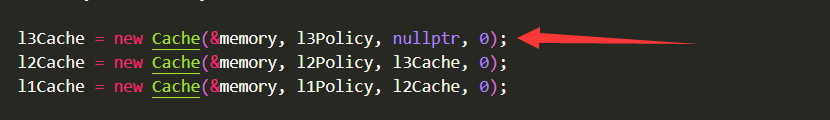
\includegraphics[scale = 0.5]{Write Policy.png}\\
The implementation of write back/through is already showed before, here is a brief introduction, each time when the cpu want to write a data, it will try to find it in the cache, if hit, the write back will modified it, set it as modified and write back it to memory at other time, the write through will both modified it and it copy in the memory. If miss, cpu will get the data from memory to the L1 and do the same thing.
\subsection{Correctness}
\subsubsection{Program Result Correctness}
This section I prove that this implementation of exclusive cache will not cause program mistake, take \textbf{quicksort.c} in test file as the example\\
Write back:\\
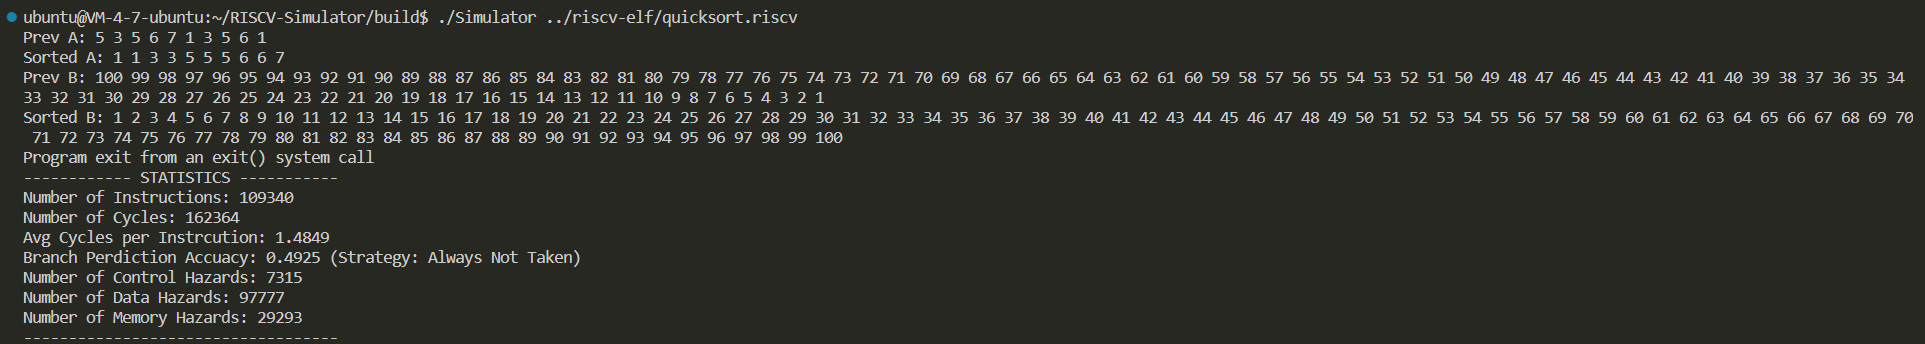
\includegraphics[scale = 0.25]{Correctness of write back.png}\\
Write through:\\
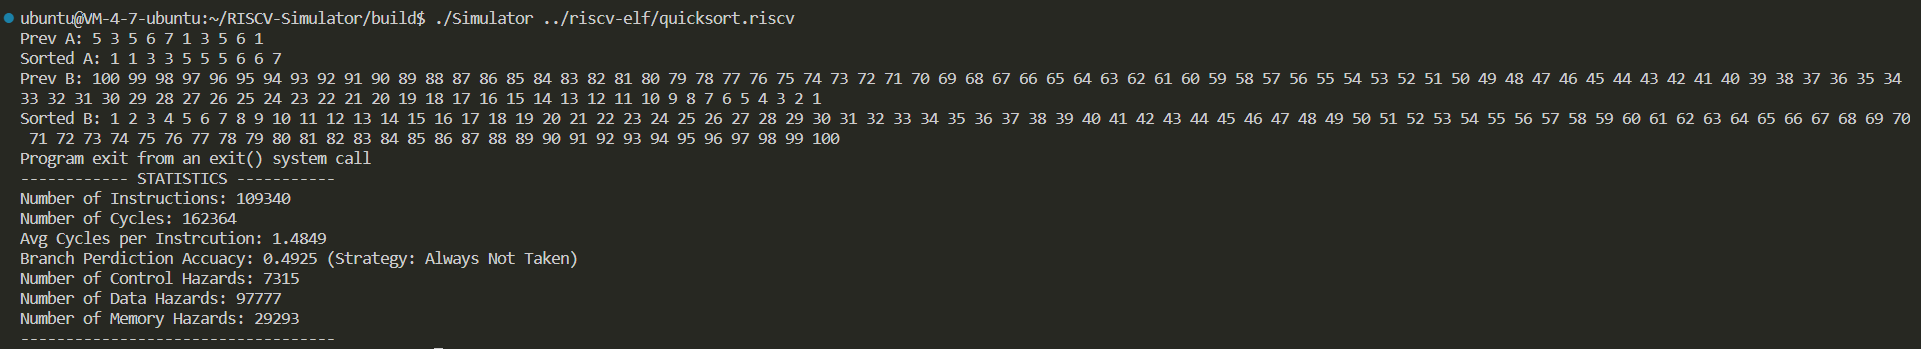
\includegraphics[scale = 0.25]{Write Through correntess.png}\\
As showed before, the implementation is correct.
\subsubsection{Cache Correctness}
To check whether the exclusive cache is implemented correctly, I add some code when there is a evit and replace happens.
\begin{lstlisting}[language=c++]
Cache *tmpcache = this->lowerCache;
while (tmpcache != nullptr)
{
    if ((blockId = tmpcache->getBlockId(addr)) != -1)
    {
        fprintf(stderr, "================error===============");
    }
    tmpcache = tmpcache->lowerCache;
}
    
\end{lstlisting}
As follows, I will check whether all other level of cache has the same copy of this block, if yes it will output error. To get a large test, I use \textbf{/cache-trace/1.trace} which has almost 10000 write and read opertion to test it. And here is the terminal output.\\
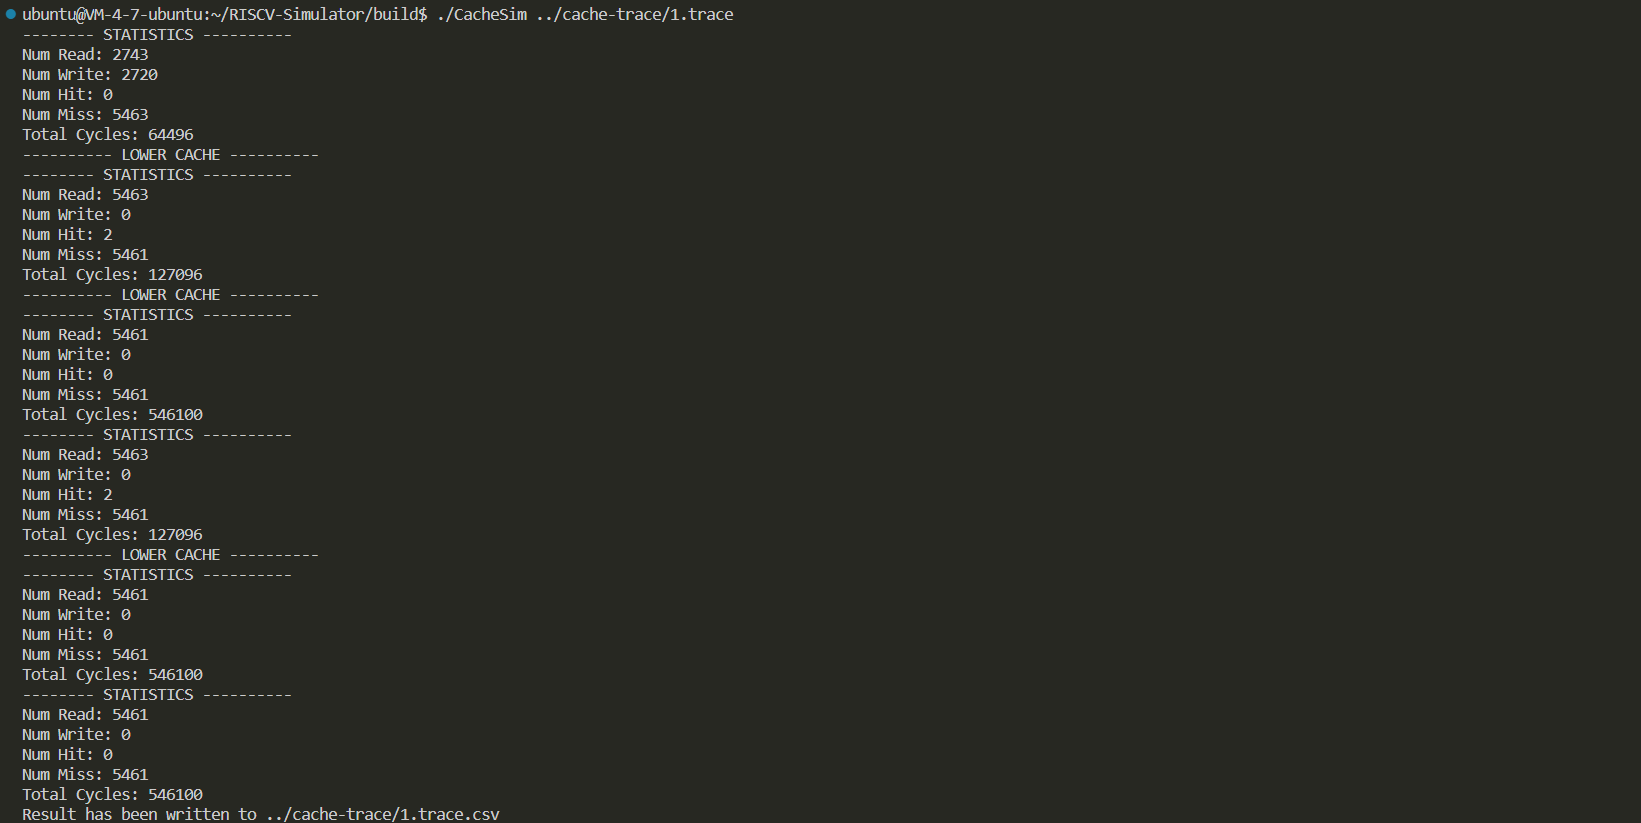
\includegraphics[scale = 0.3]{Cache correctness.png}\\
We can see there is no error ouput, which proves that my cache implementation is correct.

\subsection{Efficacy}
In this section, I propose a question of the original implementation of inclusive cache, the author read and write byte each time when visit cache, which will cause a situation, that if I want to visit an int data, the first byte of data will miss and the cache will get the block from the memory, then the remaining three bytes will get cache hit. It is odd because we should treat a cache line as a whole instead of as many bytes. The directly result is as follows,\\
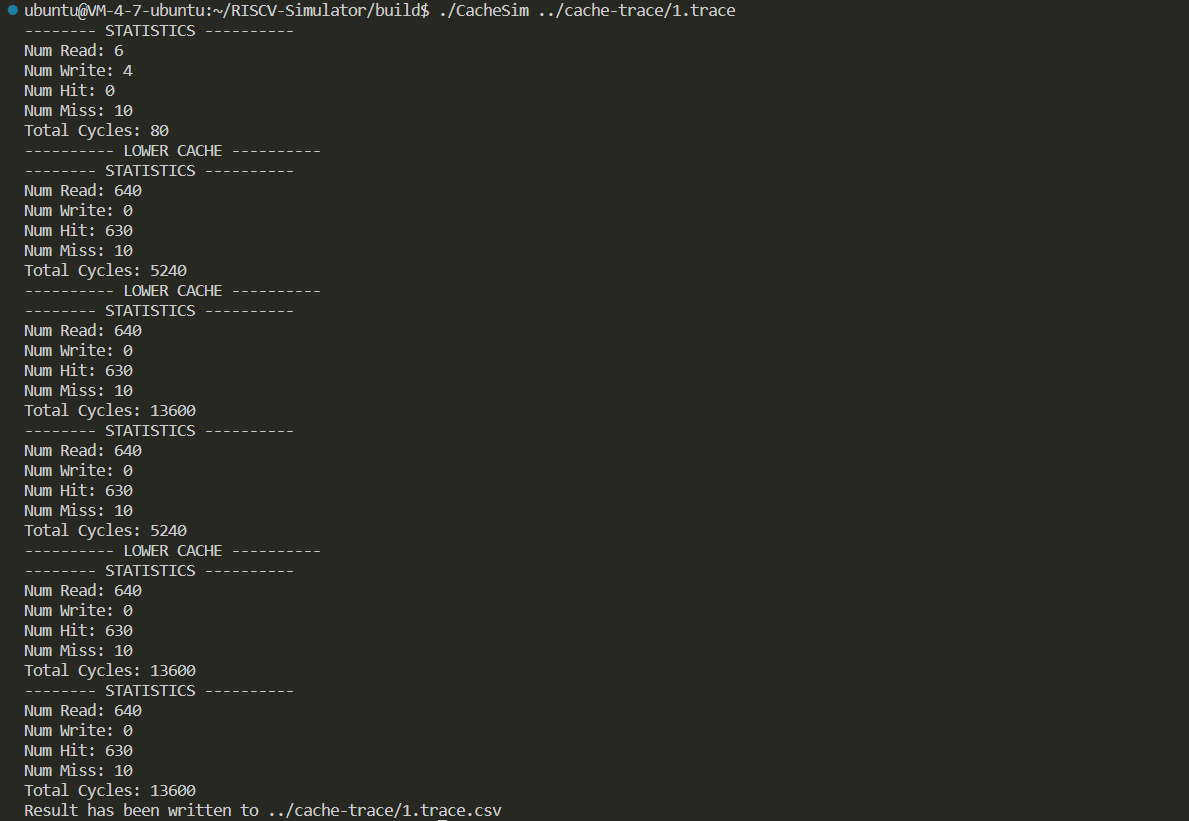
\includegraphics[scale = 0.25]{orignial cache access.png}\\
It is a kind of ridiculousness. As I only put 10 read/write in \textbf{1.trace}, there is nearly 630 hit in lower cache!\\
This is my implementation as I treat a whole cache line as a whole, the result is,\\
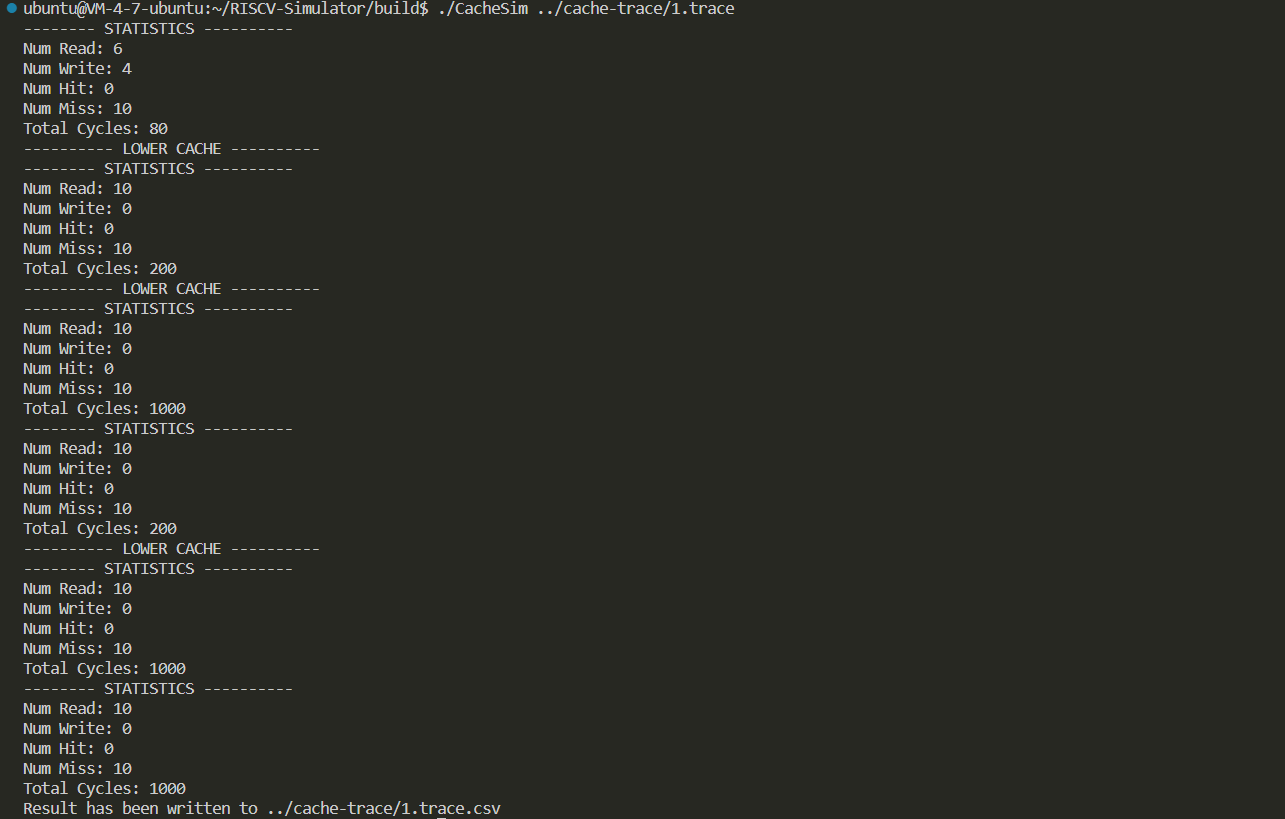
\includegraphics[scale = 0.25]{my result.png}\\
which the all cache hit in author's implementation is a cache miss at my implementation. In a word, due to the wrong implementation of the author's statistics of cache access, compare efficacy with his result is a meaningless thing.

\section{Task2}
\subsection{SDBP}
We get a \textbf{sampler tag array}, \textbf{predictor table} to help realize \textbf{SBDP}. \\
The sampler tag array is interested in, for example, 32 cache sets in LLC, has 12 entries. Each entry has 15-bit partial tags, 15-bit partial PCs, one prediction bit, one valid bit, and four bits to maintain LRU position information.\\
The predictoe table has three arrays to trace confidence, each is indexed by a hash value of blocks' signature.\\
Each time when we have a access to the LLC(a L2 cache miss)
\begin{itemize}
    \item If the block is not sampled, just do what it should do.
    \item If the block is sampled, take it's tag and the pc to the sampler
        \begin{itemize}
            \item If has already stored, add the pc to the signature, get a truncated sum
            \item If not, use LRU to replace a block, set the signature and the tag
        \end{itemize}
\end{itemize}
At the same time,
\begin{itemize}
    \item Take the tag and the PC to the predictor tables and get a confidence, compare with the threshold.
        \begin{itemize}
            \item If larger, the block is dead and will firstly replaced at next replacement.
            \item If not, nothing happens.
        \end{itemize}
\end{itemize}
Each time when we evit a block from L3 cache, which means this block is dead,
\begin{itemize}
    \item If the block is not sampled, just do what it should do.
    \item If the block is sampled, take it's tag and the pc to the sampler
        \begin{itemize}
            \item If has already stored, hash it's signature to the predictor tables, add the counter by one
            \item If not, just do what it should do
        \end{itemize}
\end{itemize}
\subsection{Implementation}
The following is new declared variables or functions to help realize \textbf{SDBP}.
\begin{lstlisting}[language=c++]
struct SamplerEntry
{
  uint32_t tag;     /* Partial tag */
  uint64_t trace;   /* Partial Signature */
  bool valid;       /* Valid bit */
  uint32_t used;    /* Refence to LRU*/
} samplerEntry;

std::vector<SamplerEntry> sampler(12);  /* Entries */
uint32_t lastRefence = 0;               /* Global refence */

/* This function is used to use LRU in entries array */
uint32_t getReplacementEntry(void)
{
  for (int i = 0; i < 12; i++)
  {
    if (sampler[i].valid = false)
    {
      return i;
    }
  }

  uint32_t min = sampler[0].used;
  uint8_t num = 0;
  for (int i = 0; i < 12; i++)
  {
    if (sampler[i].used < min)
    {
      min = sampler[i].used;
      num = i;
    }
  }
  return num;
}

/* This function is used to check whether a block 
    has already stored in entries table */
int32_t getEntryId(uint32_t tag)
{
  for (int i = 0; i < 12; i++)
  {
    if (sampler[i].tag == tag)
    {
      return i;
    }
  }
  return -1;
}

/* Entries to get confidence by hash from three table */
int32_t getConfidence(uint64_t pc, uint32_t tag)
{
  uint8_t conf1 = sample_table1[pc + tag];
  uint8_t conf2 = sample_table2[pc & tag];
  uint8_t conf3 = sample_table3[pc ^ tag];
  return (conf1 + conf2 + conf3);
}
\end{lstlisting}

The following are functions which changed.\\
\textbf{Cache::Cache} add new initialization.
\begin{lstlisting}[language=c++]
Cache::Cache(MemoryManager *manager, Policy policy, Cache *lowerCache,
    bool writeBack, bool writeAllocate)
{
  ...
  if (this->lowerCache == nullptr)
  {
    for (int i = 0; i < 12; i++)
    {
      sampler[i].valid = false;
      sampler[i].trace = 0;
      sampler[i].tag = 0;
    }
  }
  ...
}
\end{lstlisting}
\textbf{Cache::getByte}
\begin{lstlisting}[language=c++]
uint8_t Cache::getByte(uint32_t addr, uint32_t *cycles, uint64_t pc)
{
    ...
    if ((blockId = this->getBlockId(addr)) != -1)
    {
        ...
        if (this->lowerCache == nullptr)
        {   /* If it is LLC */
          int32_t tag = getTag(addr);
          uint32_t setindex = this->getId(addr);
          if ((setindex % 128) == 0)
          {  /* If it is sampled */
            int32_t EntryId;
            if ((EntryId = getEntryId(tag)) != -1)
            {   /* If in the sampler array */
              lastRefence++;
              sampler[EntryId].trace += pc;
              sampler[EntryId].used = lastRefence;
            }
            else
            {   /* If not in the sampler array */
              lastRefence++;
              EntryId = getReplacementEntry();
              sampler[EntryId].trace = pc;
              sampler[EntryId].valid = true;
              sampler[EntryId].tag = tag;
              sampler[EntryId].used = lastRefence;
            }
          }
    
          uint8_t confidence = getConfidence(pc, getTag(addr));
          if (confidence >= 8)
          { /* If larger than the threshold, dead */
            this->blocks[blockId].dead = true;
            // printf("A block is dead.\n");
          }
        }
        ...
    }
}
\end{lstlisting}
\textbf{Cache::setByte}
\begin{lstlisting}[language=c++]
void Cache::setByte(uint32_t addr, uint8_t val, uint32_t *cycles, uint64_t pc)
{
    ...
    if ((blockId = this->getBlockId(addr)) != -1)
    {
        ...
        if (this->lowerCache == nullptr)
        {   /* If it is LLC */
          int32_t tag = getTag(addr);
          uint32_t setindex = this->getId(addr);
          if ((setindex % 128) == 0)
          {  /* If it is sampled */
            int32_t EntryId;
            if ((EntryId = getEntryId(tag)) != -1)
            {   /* If in the sampler array */
              lastRefence++;
              sampler[EntryId].trace += pc;
              sampler[EntryId].used = lastRefence;
            }
            else
            {   /* If not in the sampler array */
              lastRefence++;
              EntryId = getReplacementEntry();
              sampler[EntryId].trace = pc;
              sampler[EntryId].valid = true;
              sampler[EntryId].tag = tag;
              sampler[EntryId].used = lastRefence;
            }
          }
    
          uint8_t confidence = getConfidence(pc, getTag(addr));
          if (confidence >= 8)
          { /* If larger than the threshold, dead */
            this->blocks[blockId].dead = true;
            // printf("A block is dead.\n");
          }
        }
        ...
    }
}
  
\end{lstlisting}
We update the replacement policy, since only the last level cache has dead blocks, there is no meaning to specified LLC. If there is dead block, use dead block, otherwise, still LRU policy.\\
\textbf{Cache::getReplaceBlockId}
\begin{lstlisting}[language=c++]
uint32_t Cache::getReplacementBlockId(uint32_t begin, 
    uint32_t end, uint64_t pc)
{
    /* First check invalid and dead */
    for (uint32_t i = begin; i < end; ++i)
    {
        if (!this->blocks[i].valid)
            return i;
        if (this->blocks[i].dead)
        {
            return i;
        }
    }
    
    /* Otherwise use LRU */
    uint32_t resultId = begin;
    uint32_t min = this->blocks[begin].lastReference;
    for (uint32_t i = begin; i < end; ++i)
    {
        if (this->blocks[i].lastReference < min)
        {
          resultId = i;
          min = this->blocks[i].lastReference;
        }
    }
    return resultId;
}
    
\end{lstlisting}

\subsection{Correctness}
Since the \textbf{SDBP} only change the replacement policy, I just use \textbf{quicksort.c} to test it's correctness.
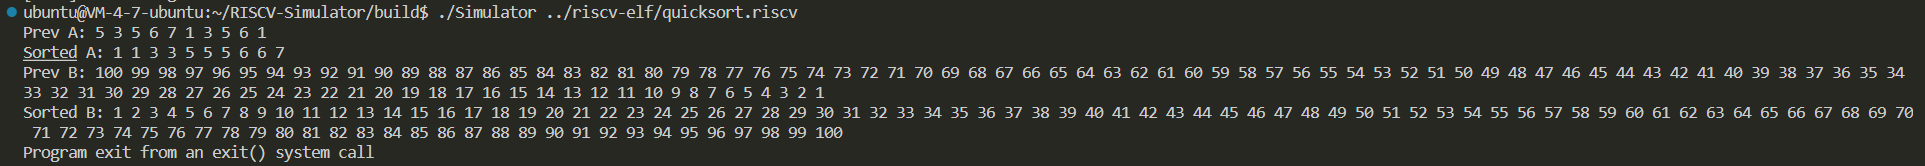
\includegraphics[scale = 0.25]{task2 correctness.png}\\

\subsection{Efficacy and Comparation}
\subsubsection{quicksort.c}
\textbf{SDBP}\\
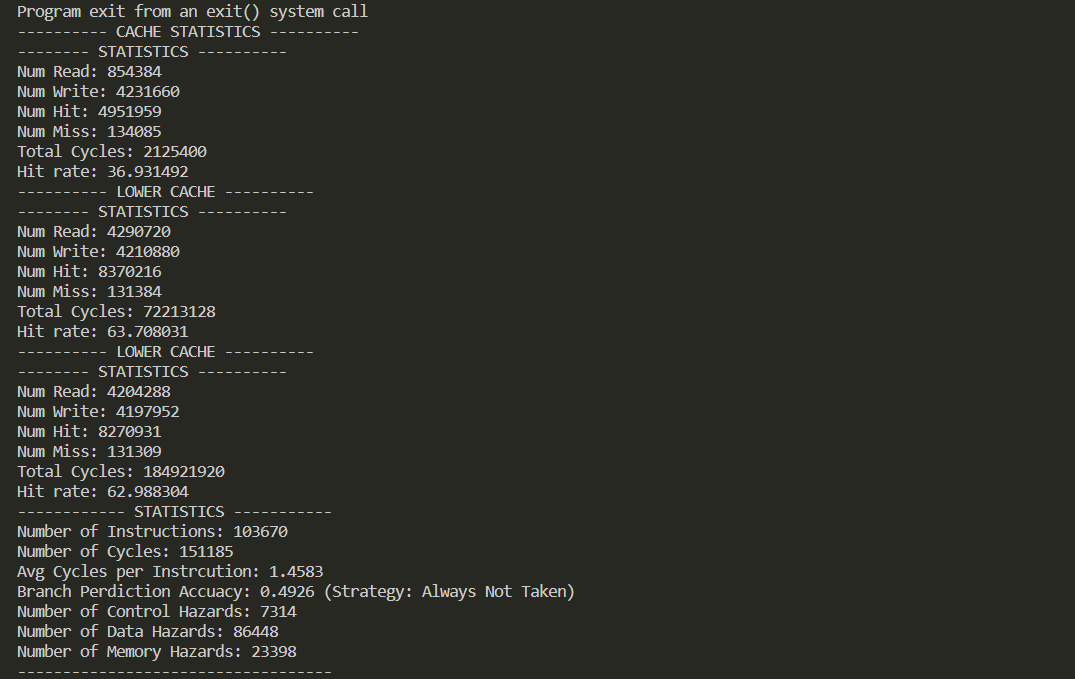
\includegraphics[scale = 0.25]{LDBP quick.png}\\
\textbf{LRU}\\
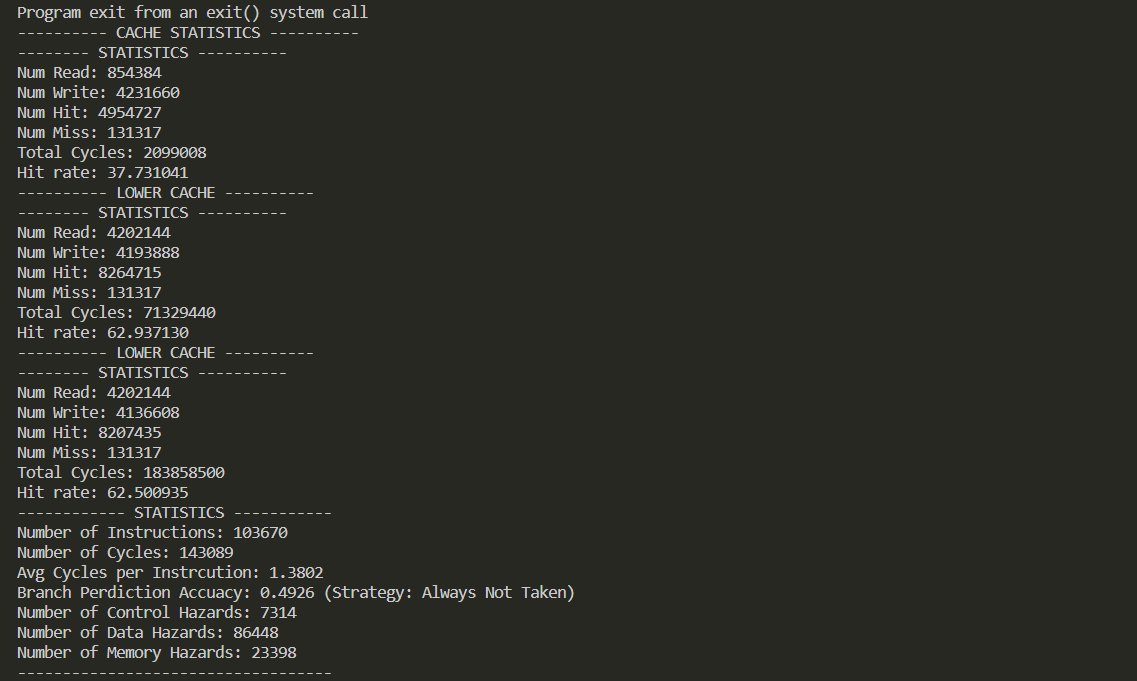
\includegraphics[scale = 0.25]{LRU quick.png}\\
\subsubsection{ackermann.c}
\textbf{SDBP}\\
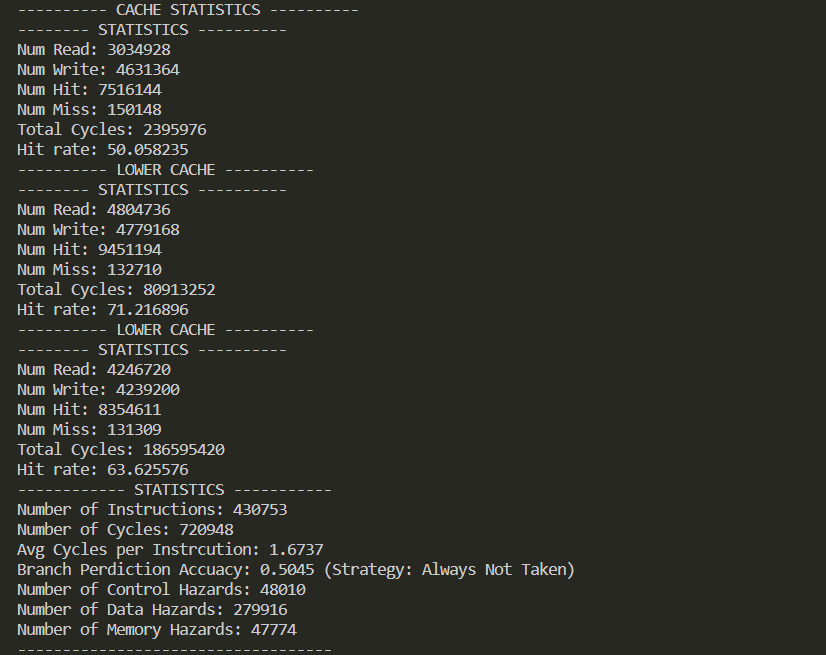
\includegraphics[scale = 0.25]{LDBP ackerman.png}\\
\textbf{LRU}\\
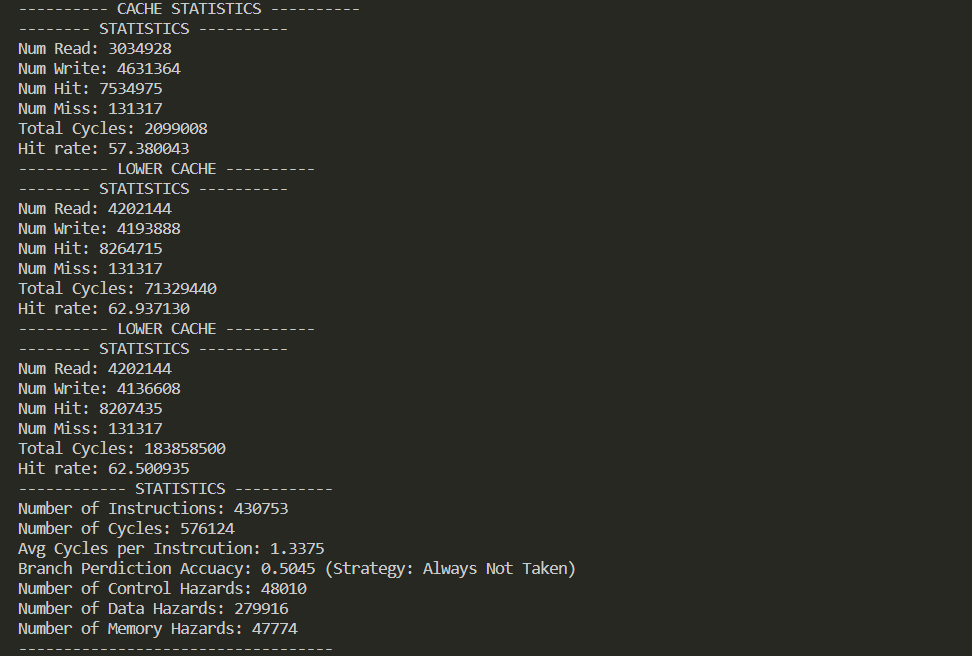
\includegraphics[scale = 0.25]{LRU achker.png}\\
\subsubsection{matrixmulti.c}
\textbf{SDBP}\\
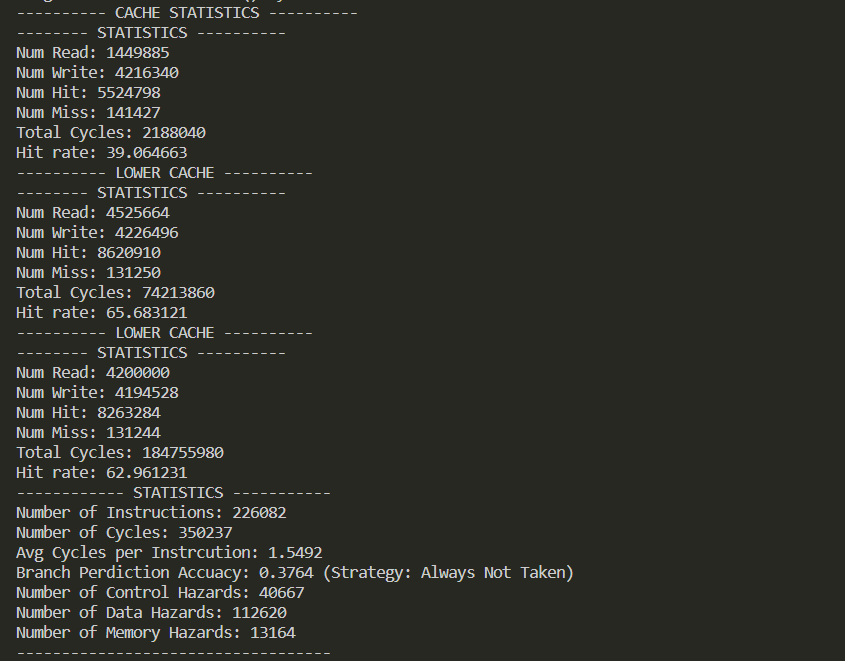
\includegraphics[scale = 0.25]{LDBP matr.png}\\
\textbf{LRU}\\
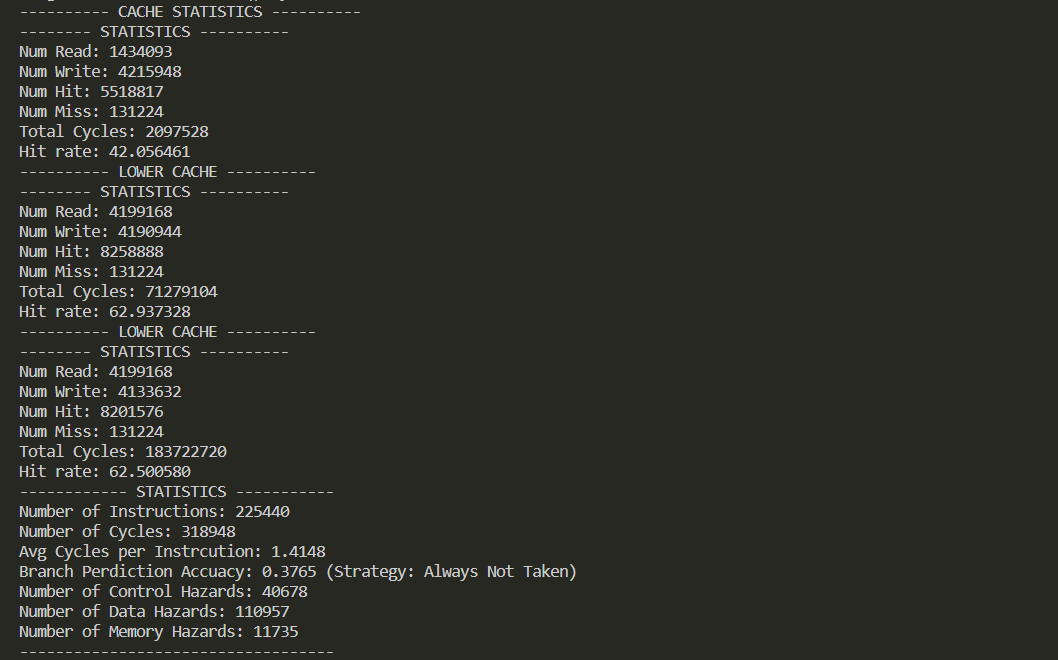
\includegraphics[scale = 0.25]{LRU matrix.png}\\

Since this we can conclude that \textbf{SDBP} can minorly improve cache efficacy.

\subsection{Some analyze and observations}
Since I'v already said the disadvantage of the miss rate calculation method before, the comparesion is a little bit meaningless, but I still observate some thing interesting.\\
First, SDBP will betterly performed compare with the LRU policy when the L1 and L2 cache is small, this is because there will more accesses to the LLC(since it is a three-level cache). \\
Also, since the three test grogramms is quite small, the differece between SDBP and LRU is reasonable not significant.\\
I also tried some other test, and I noticed that SDBP will perform worsely if the whole accesses are random and widely. This is because the sampler tag array has only 12 entries, if I randomly and widely access data, the former entries will be replaced quickly by the later entries. The SDBP will degenerate to LRU policy, but it is not a big problem at normal operating system, since many access are nearly both at space and time. But it will become a problem when there is a situation the page manager has a lot of fragmentations.
\end{document}
